\documentclass[a4paper,12pt]{article}
\usepackage{a4wide}
\usepackage[pdftex]{hyperref}
\usepackage[german]{babel}
\usepackage[utf8]{inputenc}
\usepackage{amssymb}
\usepackage{csquotes}
\usepackage{wrapfig}
\usepackage{graphicx}
\usepackage{multicol}
\usepackage{amsmath}
\usepackage{enumitem}
\usepackage{polynom}
\usepackage{siunitx}

\setlength{\marginparsep}{1 cm}
\setlength{\topmargin}{-0.6in}
\setlength{\textheight}{9.5in}
\pagestyle{plain}

\polyset{%
   style=C,
   delims={\big(}{\big)},
   div=:
}

% Polynomial long division
\polyset{%
	style=C,
	delims={\big(}{\big)},
	div=:
}

% Differential operator
\newcommand{\diff}[1]{\:\mathrm{d}{#1}}
\newcommand{\pdd}[2]{\frac{\partial #1}{\partial #2}}
\newcommand{\pddn}[3]{\frac{\partial^{#1} #2}{\partial #3^{#1}}}
\newcommand{\dd}[2]{\frac{\mathrm{d}{#1}}{\mathrm{d}{#2}}}
\newcommand{\ddn}[3]{\frac{\mathrm{d}^{#1}{#2}}{\mathrm{d}{#3^{#1}}}}

% N-th root
% \nroot{3}{27}
\newcommand*{\nroot}[2]{\sqrt[\leftroot{-1}\uproot{2}#1]{#2}}
\newcommand*{\ncroot}[4]{\sqrt[\leftroot{#1}\uproot{#2}#3]{#4}}

% 2 component vector
% \tvect{1}{-1}
% \tvec{1}{-1}
\newcommand{\tvect}[2]{%
   \ensuremath{\Bigl(\negthinspace\begin{smallmatrix}#1\\#2\end{smallmatrix}\Bigr)}}
\newcommand{\tvec}[2]{%
    \ensuremath{\left(\negthinspace\begin{matrix}#1\\#2\end{matrix}\right)}}

% 3 component vector
% \rvect{1}{-1}{0}
% \rvec{1}{-1}{0}
\newcommand{\rvect}[3]{%
   \ensuremath{\Bigl(\negthinspace\begin{smallmatrix}#1\\#2\\#3\end{smallmatrix}\Bigr)}}
\newcommand{\rvec}[3]{%
    \ensuremath{\left(\negthinspace\begin{matrix}#1\\#2\\#3\end{matrix}\right)}}

% Long vector arrow
% \xshlongvec{ABC}

% German-style quotation marks %
\MakeOuterQuote{"}

% Number sets
\newcommand{\N}{\mathbb{N}}
\newcommand{\Z}{\mathbb{Z}}
\newcommand{\Q}{\mathbb{Q}}
\newcommand{\R}{\mathbb{R}}
\newcommand{\C}{\mathbb{C}}

\newcommand{\setzero}{\varnothing}

% Mention (small caps)
\newcommand{\mention}[1]{\textsc{#1}}

% Functions
\newcommand{\asin}[0]{\text{asin}}
\newcommand{\acos}[0]{\text{acos}}
\newcommand{\atan}[0]{\text{atan}}
\newcommand{\sgn}[0]{\text{sgn}}
\newcommand{\grad}[0]{\text{grad}}

% Scale
% Usage in math mode: \Scale[1.5]{...equation...} %
\newcommand*{\Scale}[2][4]{\scalebox{#1}{$#2$}}%

% Units
\newcommand{\um}{\text{m}}
\newcommand{\us}{\text{s}}
\newcommand{\ukm}{\text{km}}
\newcommand{\ukg}{\text{kg}}
\newcommand{\uh}{\text{h}}
\newcommand{\ukmh}{\frac{\ukm}{\uh}}
\newcommand{\umpers}{\frac{\um}{\us}}
\newcommand{\umss}{\frac{\ukm}{\us^2}}
\newcommand{\ukgss}{\frac{\ukg}{\us^2}}
\newcommand{\degrees}[1]{\SI{#1}{\degree}}

% Floor / ceil
\newcommand{\floor}[1]{\left\lfloor #1 \right\rfloor}
\newcommand{\ceil}[1]{\left\lceil #1 \right\rceil}

% Circle characters
\newcommand*\circled[1]{
    \tikz[baseline=(char.base)]{
        \node[shape=circle,draw,inner sep=2pt] (char) {#1};
    }
}



\begin{document}

\begin{center}
{\bf {\large Aufgabenblatt 5 (MI/IT)}}
\end{center}

\begin{enumerate}

\item Was ist der kleinste und was der größte Wert von $x^3-x$, wenn $x$ aus dem Intervall $[-2;1]$ stammt?



\item Untersuchen Sie $-x \cdot \ln(x)$ im Intervall $(0;e]$ auf Extrem- und Wendestellen.



\item An eine zunächst unbekannte Stelle $x_0$ des Graphen von $y=\frac{1}{x}$ wird die zugehörige
Tangentengerade gelegt. Man stellt fest, dass sie die $x$-Achse bei $x=7$ schneidet. Bestimmen
Sie $x_0$!


\item Wo liegen die lokalen Minima und Maxima sowie die Wendestellen der Funktionen $\sin(x)$, $\cos(x)$,
$\tan(x)$ und $\arctan(x)$?


\item
Geben Sie irgendeine Funktion an, die ein lokales Minimum bei $x=1$ und ein lokales Maximum bei $x=2$ hat.



\item Geben Sie irgendeine Funktion an, die lokale Minima bei $x=3$ und $x=5$ hat.



\item Geben Sie eine Funktion an, deren Graph die Gerade $y=\frac{1}{2}x+3$ genau zweimal berührt. 


\item Finden Sie eine Gerade, die eine Tangente an den Graphen von $y_1=x^2$ und zugleich eine an den Graphen
von $y_2=-x^2+5x-17/4$ ist.


\end{enumerate}

\vspace{1cm}

Rätselaufgabe: Es geht die Rede, dass drei Nachbarn, die gemeinsam einen kleinen Park hatten, so wie im Bild zu sehen ist, Streit bekamen. Der Besitzer des großen Hauses beklagte sich über die Hühner seiner Nachbarn, die ihn störten, und baute von seiner Tür zum Tor vorn im Bild einen abgegrenzten Weg. Daraufhin baute der Mann in dem Haus rechts einen Weg zum Tor auf der linken Seite und der Mann in dem Haus links einen Weg zum Tor auf der rechten Seite.
Die Wege kreuzten sich an keiner Stelle. Können Sie alle drei richtig einzeichnen?

\begin{figure}[ht]
	\centering
  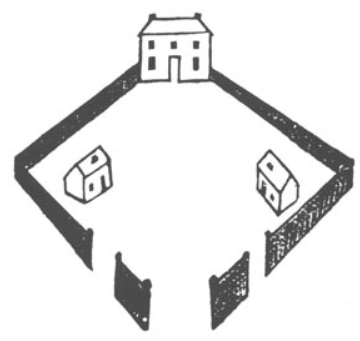
\includegraphics[width=0.3\textwidth]{../pool/ex-graph-theory-1-img-a.png}
%	\caption{}
	\label{fig1}
\end{figure}



\newpage

\begin{center}
{\bf {\large Lösungen}}
\end{center}

\begin{enumerate}

\item

Kandidaten für den höchsten und kleinsten Wert sind die Grenzen des Intervalls $[-2;1]$ sowie die lokalen Extrempunkte.

$f'(x) = 3x^2-1 = 0$

$\implies 3x^2 = 1$

$\implies x_{1,2} = \pm \frac{\sqrt{3}}{3}$

Es gilt $1 = \sqrt{1} < \sqrt{3} < \sqrt{4} = 2$, also $\frac{\sqrt{3}}{3} \in [\frac{1}{3}; \frac{2}{3}]$, die Kandidaten für Extrempunkte $x_{1,2}$ liegen also im betrachteten Intervall.

Nun rechnen wir die Funktionswerte an den Intervallgrenzen und an den möglichen Extremstellen aus:

$f(-2) = (-2)^3 + 2 = -6$

$f(1) = 1^3 - 1 = 0$

$f(\frac{\sqrt{3}}{3}) = 3*\frac{\sqrt{3}}{27} - \frac{\sqrt{3}}{3} = -\frac{2}{9}\sqrt{3}$

$f(-\frac{\sqrt{3}}{3}) = -3*\frac{\sqrt{3}}{27} + \frac{\sqrt{3}}{3} = \frac{2}{9}\sqrt{3}$

Nach obiger Abschätzung ergibt sich wieder $\frac{2}{9}\sqrt{3} \in [\frac{2}{9};\frac{4}{9}]$, somit ist der kleinste Wert $-6$ und der größte Wert $\frac{2}{9}\sqrt{3}$.



\item

Zuerst Ableiten:

$f'(x) = -\ln(x)-1$

$f''(x) = -1/x$

$f'''(x) = 1/x^2$

Kandidaten für Extremstellen durch $f'(x) = 0$

$-ln(x) - 1 = 0$

$\implies \ln(x) = -1$

$\implies x = \frac{1}{e}$

Prüfen ob Minima oder Maxima durch Einsetzen in 2. Ableitung:

$f''(\frac{1}{e}) = -e < 0 $

Also Maxima bei $x=\frac{1}{e}$

Kandidaten für Wendepunkte durch $f''(x) = -1/x = 0$. Diese Gleichung ist nicht lösbar, also keine Wendepunkte.



\item

Wir berechnen die Gleichung der Tangentengerade in Abhängigkeit vom Anlagepunkt $x_0$.

Der Anstieg $m$ der Tangenten folgt aus der 1. Ableitung:

$f'(x) = -\frac{1}{x^2}$

$\implies f'(x_0) = -\frac{1}{x_0^2}$

Der Funktionswert an der Stelle $x_0$ ergibt sich zu $f(x_0) = \frac{1}{x_0}$. Die Tangentengleichung $t(x)$ lautet somit:

$t(x) = f(x_0) + f'(x_0) (x-x_0) = \frac{1}{x_0} -\frac{1}{x_0^2} (x-x_0)$

Die Tangente schneidet die x-Achse in der Nullstelle $x_z$:

$t(x_z) = 0 = \frac{1}{x_0} -\frac{1}{x_0^2} (x_z-x_0)$

$\implies \frac{1}{x_0} = \frac{1}{x_0^2} (x_z-x_0) $

$\implies x_0 = x_z-x_0 $

$\implies x_z = 2x_0 $

Nach Aufgabestellung soll der Schnittpunkt der Tangente mit der x-Achse bei $7$ liegen, also $x_z = 2x_0 = 7$, somit $x_0 = 3.5$.



\item

Hinweis: 

$\frac{d}{dx}\tan(x) = \frac{1}{\cos^2(x)}$

$\frac{d}{dx}\text{atan}(x) = \frac{1}{x^2+1}$

Unter Kentniss der Winkelfunktionen erhält man:

\begin{itemize}
\item $\sin(x)$: Minima bei $\frac{3}{2}\pi+2\pi{n}$, Maxima bei $\frac{\pi}{2}+2\pi{n}$, Wendepunkte bei $\pi{n}$, $n \in \mathbb{Z}$
\item $\cos(x)$: Minima bei $\pi+2\pi{n}$, Maxima bei $2\pi{n}$, Wendepunkte bei $\frac{\pi}{2}+\pi{n}$, $n \in \mathbb{Z}$
\item $\tan(x)$: keine (lokalen) Minima oder Maxima, Wendepunkte bei $\pi{n}$, $n \in \mathbb{Z}$
\item $\text{atan}(x)$: keine (lokalen) Minima oder Maxima, Wendepunkt bei $x=0$
\end{itemize}



\item Es sind verschiedene Arten von Funktionen möglichen. Im Folgenden zwei Ansätze, eine solche Funktionsgleichung aufzustellen:

\begin{enumerate}

\item Ansatz 1: Kubische Funktion. An Minima und Maxima ist die Ableitung 0. Die Ableitung der kubischen Funktion ist also eine Parabel mit den Nullstellen 1 und 2:

$f'(x)=-(x-1)\cdot(x-2)$

Ausmultiplizieren und ableiten:

$f'(x)=-(x-1)\cdot(x-2)= -(x^2-2x-x+2)=-x^2+3x-2$.

$f''(x) = -2x+3$

Da $f''(1) = -2*1+3 = 1 > 0$ liegt bei $x=1$ ein Minima vor und wegen $f''(2) = -2*2+3 = -1 < 0$ bei $x=2$ ein Maxima.

Nun integrieren, um die kubische Funktion zu erhalten:

$f(x) = -\frac{1}{3}x^3+\frac{3}{2}x^2-2x+C$

Für $C$ kann eine beliebige reele Zahl eingesetzt werden.

\item Ansatz 2: Sinus-Funktion

$f(x)=-\sin(\pi \cdot (x-\frac{1}{2}))$

Die Periode obiger Sinus-Funktion ist $\frac{2\pi}{\pi} = 2$. Sie zudem um $1/2$ nach rechts verschoben und an der x-Achse gespiegelt, hat damit also ein Minimum bei $1$ und ein Maxima bei $2$.

\end{enumerate}



\item Analog zur 1. Aufgabe.

\begin{enumerate}

\item Ansatz 1: Polynom 4. Grades mit 2 Nullstellen der Vielfachheit 2.

$f(x) = (x-3)^2(x-5)^2$

Wir überprüfen noch, ob es sich um Minima oder Maxima handelt. Ableiten:

$f'(x) = 2(x-3)(x-5)^2+2(x-3)^2(x-5) = 2(x-3)(x-5)*((x-5)+(x-3)) = 2(x-3)(x-5)(2x-8)$

(Die Ableitung hat also Nullstellen bei $3$ und $5$, zudem auch noch bei $4$).

Nochmal Ableiten und die Kandidaten für die Minima einsetzen:

$f''(x) = 2*((x-5)(2x-8)+(x-3)(2x-8)+(x-3)(x-5))$

$f''(3) = 2*((3-5)(6-8)) = 8 > 0$

$f''(5) = 2*((5-3)(10-8)) = 8 > 0$

$f''(4) = 2*((4-3)(4-5)) = -2 < 0$

Die Funktion $f(x) = (x-3)^2(x-5)^2$ hat also Minima bei $3$ und $5$ sowie ein Maxima bei $4$.

\item Ansatz 2: Cosinus-Funktion

$f(x) = -cos(\frac{\pi}{2}*(x-3))$

\end{enumerate}



\item

Gegeben ist die Gerade $f(x) = \frac{x}{2}+3$. Sie hat den y-Achsenschnittpunkt $f(0) = 3$ und die Nullstellen $x_0 = -6$. Ihre Ableitung (Anstieg) ist $\frac{1}{2}$.

Wir suchen eine Funktion, die etwa zweimal von oben auf die Gerade eingeht. Wir setzen an mit einem Polynom $p$ vom Grade 4:

$p(x) = x^4+ax^3+bx^2+cx+d$

Wir betrachten die beiden Stellen $0$ und $-6$. Dort müssen die Funktionswerte und die ersten Ableitungen übereinstimmen:

$p(0) = 3$

$p'(0) = \frac{1}{2}$

$p(-6) = 0$

$p'(-6) = \frac{1}{2}$

Aus der ersten Bedinung folgt $p(0) = d = 3$ und aus der zweiten $p'(0) = c = \frac{1}{2}$. Somit hat $p$ die Form

$p(x) = x^4+ax^3+bx^2+\frac{x}{2}+3$

$p'(x) = 4x^3+3ax^2+2b+\frac{1}{2}$

Wir setzen die letzten beiden Bedinungen ein:

\begin{enumerate}
\item $p(-6) = 0 = 1296 - 216a + 36b$
\item $p'(-6) = \frac{1}{2} = -864 + 108a -12b + \frac{1}{2}$
\end{enumerate}

Dies stellt ein lineares Gleichungsystem dar. Wir können es etwa lösen, indem wir Gleichung $(b)$ mit $3$ multiplizieren und zur Gleichung $(a)$ addieren:

$-1296+108a = 0$
$\implies a=12$

Es folgt aus Gleichung $(b)$

$12b = 108a-864 = 432$
$\implies b=36$

Die Funktionsgleichung lautet somit

$p(x) = x^4 + 12x^3+36x^2+\frac{1}{2}x+3$



\item

Gegeben sind die beiden Funktionen mit ihren Ableitungen:

$f_1(x) = x^2$

$f_2(x) = -x^2+5x-\frac{17}{4}$

$f_1'(x) = 2x$

$f_2'(x) = -2x+5$

Wir betrachten die Tangente $t_1$ an $f_1$ an der Stelle $x_1$; und die Tangente $t_2$ an $f_2$ an der Stelle $x_2$. Wir wollen die 2 Stellen $x_1$ und $x_2$ so bestimmen, dass die Tangenten $t_1$ und $t_2$ gleich sind.

Insbesonders müssen also ihre Anstiege gleich sein:

$f_1'(x_1) = f_2'(x_2)$

$\implies 2x_1 = -2x_2+5$

$\implies x_1 = \frac{5}{2}-x_2$

Diese Beziehung nutzen wir später. Wir bilden die Tangente an $f_1$:

$t_1(x) = f_1(x_1) + f_1'(x_1)(x-x_1) = t_1(x) = x_1^2+2x_1(x-x_1)$

Da die Tangenten gleich sein sollen, muss der Funktionswert der Tangente $t_1$ im Punkt $x_2$ gleich dem Funktionswert der Funktion $f_2$ sein, also $t_1(x_2)$ = $f_2(x_2)$. Wir betrachten zuerst $t_1(x_2)$:

$t_1(x_2) = x_1^2+2x_1(x_2-x_1) =-x_1^2+2 x_1 x_2$

Da nun gilt $x_1 = \frac{5}{2}-x_2$:

$t_1(x_2) = -(\frac{5}{2}-x_2)^2+2(\frac{5}{2}-x_2)x_2 =-3x_2^2+10x_2-\frac{25}{4}$

Wie erwähnt muss gelten $t_1(x_2)$ = $f_2(x_2)$:

$t_1(x_2)$ = $f_2(x_2)$

$\implies -3x_2^2+10x_2-\frac{25}{4} = -x_2^2+5x_2-\frac{17}{4}$

$\implies -2x_2^2+5x_2-2 = 0$

$\implies x_2^2-\frac{5}{2}x_2+1 = 0$

$\implies x_2 = \frac{5}{4} \pm \sqrt {\frac{25}{16}-1} = \frac{5}{4} \pm \sqrt {\frac{9}{16}} = \frac{5}{4} \pm \frac{3}{4}$

$\implies x_2 = \frac{1}{2} \lor x_2 = 2$

Da $x_1 = \frac{5}{2}-x_2$, folgt auch $x_2 = \frac{1}{2} \lor x_2 = 2$. Es gibt also zwei mögliche Tangenten, diese lauten:

$t_1(x) = \frac{1}{4} + (x-\frac{1}{2})$

$t_2(x) = 4 + 4(x-2)$



\newpage

Knobelaufgabe:

\begin{figure}[ht]
	\centering
	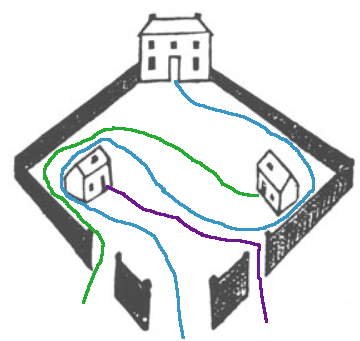
\includegraphics[width=0.3\textwidth]{../tex-snippets/ex-graph-theory-1-img-b.png}
	\label{knobel}
\end{figure}



\end{enumerate}

\end{document}

